\documentclass[openany]{UoYCSproject}

\protect\BEng
\protect\supervisor{Dr William Smith}
\protect\wordcount{(to-be-completed)}
\protect\includes{the title page and the abstract}
\protect\excludes{bibliographies and appendices}
\protect\abstract{This project produces a functional web application to visualise potential avalanche hazards. Within a virtual 3D terrain reality, avalanche hazards along popular winter mountaineering routes can be observed. The project has a primary focus on Scottish mountains while providing excellent adaptability for other regions with appropriate data sources. Avalanche hazards were calculated from a combination of professional avalanche forecasts and spatial analysis of mountain terrain models. Both the accuracy and the usability of the application were evaluated through statistical comparisons with past avalanche records and user experimentation. Additional features such as locating historical avalanches and route planning are also provided in the application. The safety and ethical considerations of the application being put into real world use are discussed.}

\usepackage[left=26mm,top=26mm,right=26mm,bottom=26mm]{geometry}    
\geometry{a4paper}
\usepackage{algorithm,algpseudocode}     
\algnewcommand\Or{\textbf{ or }}   
\algnewcommand\In{\textbf{ in }}   
\algnewcommand\NotIn{\textbf{ not in }} 
\makeatletter
\renewcommand{\ALG@beginalgorithmic}{\small}
\makeatother     		
\usepackage{graphicx}					
\usepackage{amssymb}
\usepackage{amsmath}
\usepackage{gensymb}
\usepackage{url}
\usepackage[parfill]{parskip}
\usepackage{natbib}
\usepackage{array}
\usepackage{color}
\usepackage[usenames,dvipsnames,svgnames,table]{xcolor}
\setlength{\headsep}{7pt}
\graphicspath{ {images/} }
\setlength{\bibsep}{3pt plus 3ex}
\definecolor{notapplicable}{RGB}{192,192,192}
\definecolor{low}{RGB}{153,255,153}
\definecolor{moderate}{RGB}{255,255,153}
\definecolor{considerable}{RGB}{255,178,102}
\definecolor{high}{RGB}{255,102,102}
\definecolor{veryhigh}{RGB}{102,0,0}
\definecolor{notapplicable-new}{RGB}{255, 255, 255}
\definecolor{low-new}{RGB}{255, 255, 112}
\definecolor{moderate-new}{RGB}{230, 172, 0}
\definecolor{considerable-new}{RGB}{255, 127, 0}
\definecolor{high-new}{RGB}{255, 0, 0}
\definecolor{veryhigh-new}{RGB}{128, 0, 0}

\title{An App for Visualisation of Avalanche Hazard}
\author{Chongyang Shi}
\date{(to-be-completed)}							
\begin{document}

{\let\cleardoublepage\clearpage 
    \maketitle
}

\chapter{Introduction}

\section{Overview of the project}

The purpose of this project is to produce a functional web application to visualise potential avalanche hazards. The application is to work on both desktop and mobile devices. Through the application, the user is able to freely explore the virtual 3D terrain reality and observe avalanche hazards along popular mountaineering routes. Useful tools such as a route planner and a past avalanche locator are also included in the application.

A model for calculating localised avalanche hazards based on carefully sourced and processed avalanche forecasts \cite{sais} and terrain model data \cite{os-5} was produced by the project. The accuracy of the model has been statistically evaluated against past avalanche records \cite[pp. 143-151]{scottish-avalanches}\cite{sais-map}. Usability and effectiveness of the application guiding the user away from hazardous locations were evaluated through test uses conducted with experienced mountaineers. 

The project incorporated tools and techniques from various aspects of Computer Science, including software engineering, geographic information system (GIS) modelling, human-computer interaction, computer graphics and algorithms. Many of these tools and techniques are associated with current research in these areas.

\section{Motivations behind the application}

As a front-runner of digital avalanche forecasts, the Scottish Avalanche Information Service (SAIS) \cite{sais} have been providing frequent and reliable winter avalanche forecasts for decades in Scotland.

In addition to written observations on conditions of the snowpack and weather, a typical SAIS avalanche forecast also includes a compass rose, providing avalanche risk levels on the scale of 1 to 5 for slopes of different aspects above and below a transition threshold altitude, shown in Figure \ref{fig:mapping}. However, while this compass rose provides a comprehensive overview on avalanche risks across the forecast region, it is not straightforward to interpret, as the user will need to work out the surface aspects and altitudes along their route, and mentally infer the risk levels of different locations along their route. This is a very complex task, as it is not only easy to underestimate the risk due to risk levels varying sharply between neighbouring aspects and altitudes (as shown in Figure \ref{fig:mapping}), but also requires the user not to be unnecessarily cautious to avoid better routes with less risk than the user believes. 

Therefore, the primary purpose of this project is to vastly simplify this process, by generating a coloured image based on the altitude and surface aspects at each point (as determined by a terrain height-map raster), which is then laid on top of a computer-generated terrain model in the 3D terrain viewer. Hence the information supplied by the compass rose can be visualised in the most straightforward way, allowing the user to freely navigate the 3D model and observe the hazard levels at each location along their route. The avalanche hazard of the same area mapped in Figure \ref{fig:mapping} is visualised as shown in Figure \ref{fig:stage1bennevis} (also shown on the right is the final product with high risk terrain areas accentuated and an improved colour coding).

In later stages of the project, we also seek to improve hazard representation through constructing a custom risk model based on information from the compass rose and terrain spatial data; and to improve the functionalities of the application by adding in features such as pathfinding.

\begin{figure}[h]
		\centering
		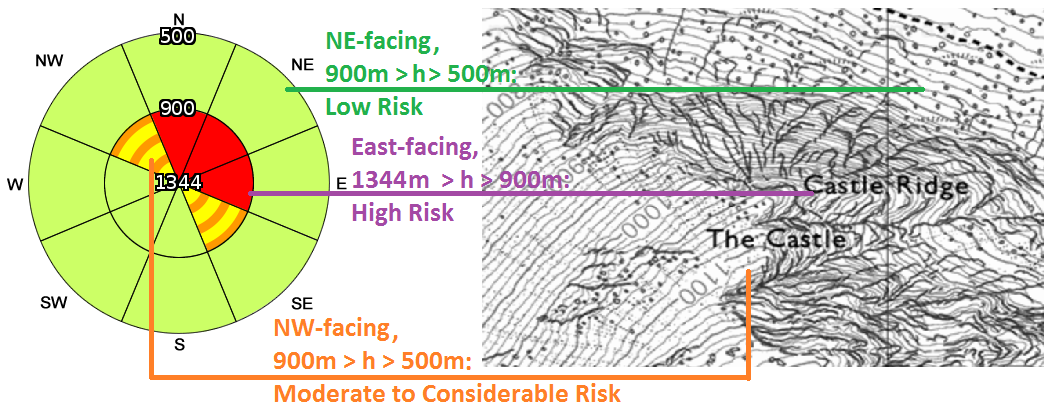
\includegraphics[scale=0.9]{Mapping.png}
		\caption{\label{fig:mapping} An example compass rose produced by the SAIS on January 6, 2016 for Lochaber (left), showing a steep transition of risk levels; and an example manual inference of risk levels based on the compass rose and contour lines near Ben Nevis, Lochaber (right).  \cite{sais-lochaber0106}}
\end{figure}

\begin{figure}[h]
		\centering
		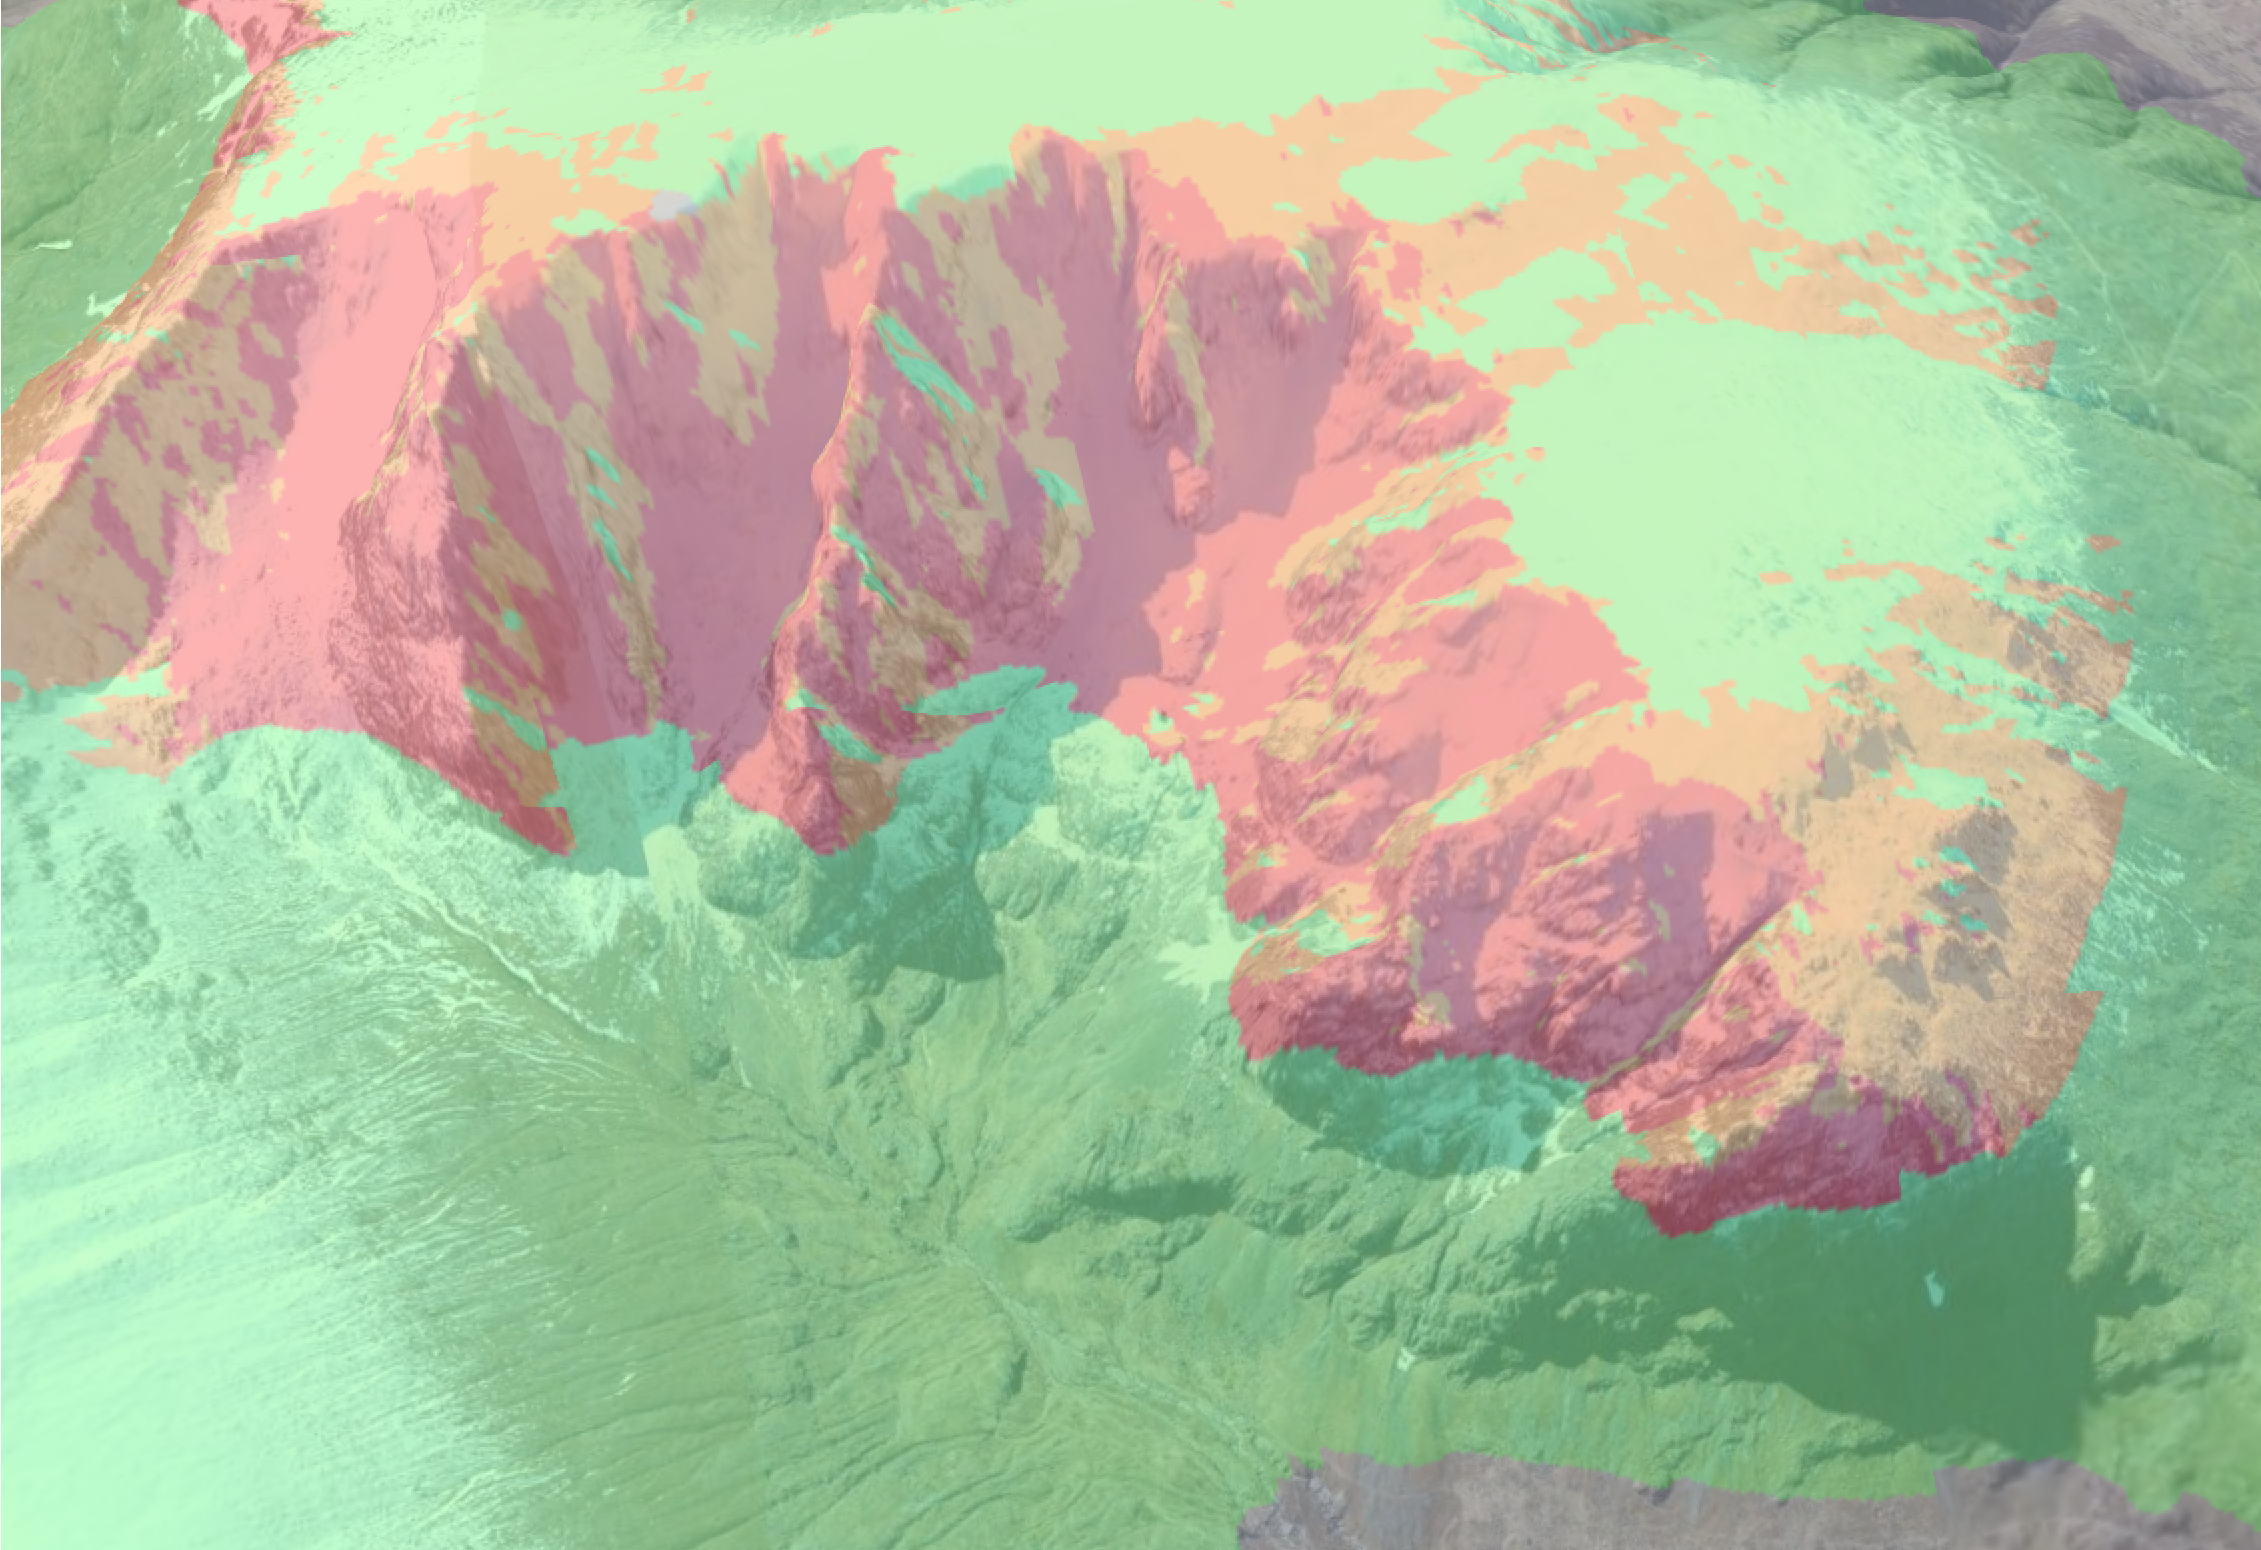
\includegraphics[height=4.5cm]{Stage1BenNevisRight.png}
		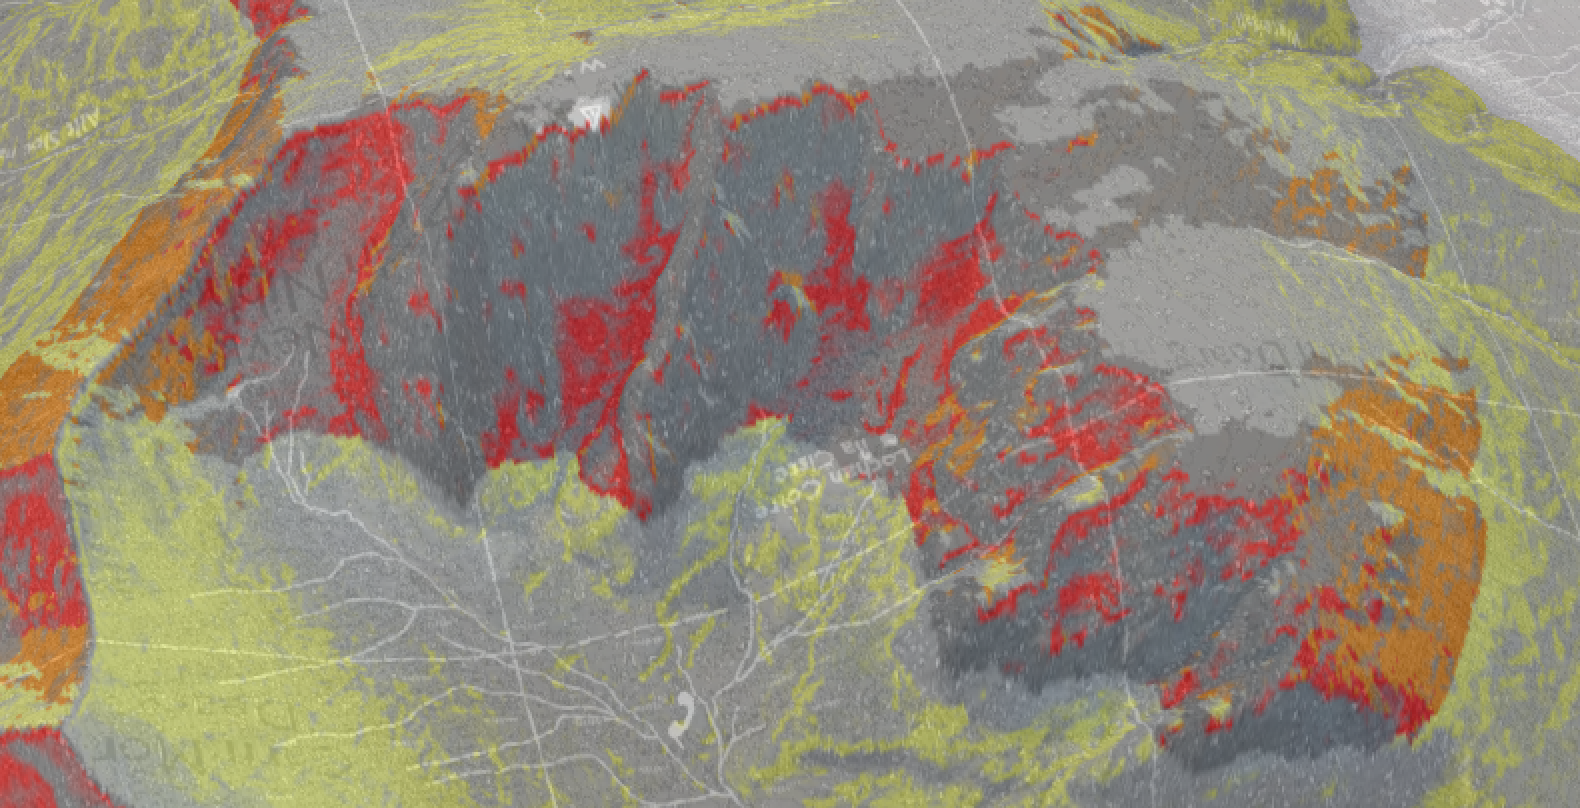
\includegraphics[height=4.5cm]{Stage3BenNevis.png}
		\caption{\label{fig:stage1bennevis} The avalanche hazard visualisation of the same area mapped in Figure \ref{fig:mapping}, generated in the 3D terrain viewer using the same avalanche forecast by both the basic product (dynamic risk only, left) and the final product (both static terrain and dynamic risk with new colour coding, right).}
\end{figure}



\section{Stages of the project}

The course of the project was divided into a preliminary stage and four development stages, in order to effectively track and manage the workload. As the product from each stage is able to function independently of work done in later stages, unforeseen difficulties encountered in the research and development process can be effectively mitigated. The stages are described as followed:

\textbf{Preliminary Stage - Requirement Gathering:} As a preparation for the software development, some analysis were performed on the project specification and stakeholders were interviewed in order to gather requirements for the application. In particular, potential users were inquired about how they access and use avalanche forecasts at the time, and what improvements could the application of the project bring.

\textbf{Stage 1 - Basic Functionalities:} The aim of this stage was to select appropriate application frameworks and libraries to produce a basic but functional application: a 3D terrain viewer with a hazard map overlay, the data for which would be derived solely from forecasts by the Scottish Avalanche Information Service \cite{sais}. The WebGL framework Cesium \cite{cesium} was chosen as the foundation for front-end developments, while Python was chosen for developing the backend, and to interface other systems such as GIS processors with its vast range of interfacing libraries.

\textbf{Stage 2 - Improved Spatial Analysis and Evaluation:} This stage of the project extends the data source for the hazard map overlay by performing surface fitting and spatial analysis on the terrain model data \cite{os-5}, in order to make the hazards more localised and to better reflect the hazard posed by unique terrain features such as concave slopes. MATLAB \cite{matlab-primer} and other GIS tools were used to perform the computations for these purposes. Evaluations on the localised hazard map against avalanche records were also conducted at this stage, with a focus on the avalanche ``blackspots'' of Scottish mountains.

\textbf{Stage 3 - Risk-adjusted Pathfinding:} With a localised hazard map obtained in Stage 2, this stage was focused on developing a pathfinding tool for the front end application, allowing the user to plot a potential hiking path with a configurable avalanche risk level. Techniques such as A* path finding \cite{cui2011based} were utilised to develop this functionality. 

\textbf{Stage 4 - Usability Testing:} The final stage of the project focus on the human-computer interaction aspects of the application. Experienced mountaineers were consulted and invited to test use the application and to provide feedback on usability as well as the effectiveness of the application guiding them away from avalanches that would have occurred in real use. Some improvements were made based on the feedbacks.

\section{Considerations and statements on ethics}

The application was designed as a tool to improve winter mountaineering safety, therefore evidently the foremost consideration on ethics is regarding the accuracy and robustness of avalanche hazards projected by the application. If a location with imminent avalanche threat is reported as safe by the application, a user relying on the guidance of this application could be placed in serious danger; conversely, if the application indicate avalanche warnings to users at a location where an avalanche is unlikely to occur, undue anxiety could be caused.

Due to the constraints placed on the lifecycle of this project, it is difficult to conduct an extensive peer review process to examine the accuracy of hazard projections. And while most open source libraries used during the development process are widely-used and have been well-tested, software errors may still occur and affect the safety assurance of the product. Furthermore, the lack of a known commercial or academic product with comparable functionalities eliminates the possibilities of cross-testing the software product.

As a result, while the application is functional and has shown promise during our own evaluations, it is not considered as a product ready for real-life use -- a warning of which is displayed when a user accesses the application.

\section{Structure of this report}

A literature review is conducted in Chapter \ref{ch:lit-review} over existing research and developments in the various aspects of Computer Science involved in this project. Theories studied and developed for the development of the application as well as the processing of available data are discussed in Chapter \ref{ch:theory}. Chapter \ref{ch:app-description} describes in detail the features and internal architectures of the application, as well as its development process. This is followed by Chapter \ref{ch:app-testing}, which describes the evaluation and testing conducted on the application as well as on the quality of its data. Finally, Chapter \ref{ch:conclusions} concludes the report and discusses the potential uses and future developments of the application.

\chapter{Literature Review} \label{ch:lit-review}

As an application designed to improve the usability of snow avalanche forecasts, it is necessary to first consider and evaluate past research and efforts made to understand and predict avalanches, as well as efforts in visualising these knowledge and predictions. While the term avalanche can be applied to various types of moving substances, such as rock and mud \cite[p. 1]{91097820150101}, only snow avalanches are studied by this project.

The literature review starts with an overview of the cause, classification and consequences of snow avalanches in Section \ref{sec:avalanche-background} to motivate the need of accurately visualising avalanche risks. This is followed by comparisons and critiques on existing methods and models for forecasting avalanches in Section \ref{sec:avalanche-forecasting}, which can be potentially applied in analysing avalanche forecasts and topographical data in Chapter \ref{ch:theory}. Past efforts in modelling and visualising avalanches risks are then discussed in Section \ref{sec:modelling-avalanche}, which provides reference theories in designing risk analysis models used in Chapter \ref{ch:theory}. Section \ref{sec:colour-representation} looks into the theories behind colour representations of risk, providing a basis for the colour design of the visualisation in Chapters \ref{ch:theory} and \ref{ch:app-description}. Section \ref{sec:terrain-pathfinding} discusses existing methods in cost calculations in 3D space, and compares researches in the pathfinding algorithm A*, for algorithmic designs of the route planning tool in Chapter \ref{ch:app-description}. Finally, Section \ref{sec:application-usability} covers existing Human-computer Interaction researches in 3D navigation and field usage required by the project, which provides background and guidance to evaluations conducted in Chapter \ref{ch:app-testing}.

\section{Background on snow avalanches} \label{sec:avalanche-background}

Accumulated snow is usually not a stable structure -- snow found in avalanches are usually 80\% air, and the snow cover gradually deforms as environment temperature approaches the melting point of snow \cite[p. 16]{mcclung2006avalanche}. This instability fundamentally allows frequent occurrence of avalanches. 

Snow avalanches occur when large masses of snow or ice move rapidly down a mountainside or over a precipice, often triggered from the snow cover \cite[p. 1]{91097820150101}. Avalanches can either be triggered naturally due to combinations of certain geographical \cite[p. 17]{91097820150101} and meteorological \cite[p. 23]{91097820150101} conditions, or triggered by human activities nearby \cite{schweizer2001characteristics}. Often the latter is constructive to the former when an avalanche is triggered \cite[p. 17]{mcclung2006avalanche}\cite[p. 48]{scottish-avalanches}.

McClung and Schaerer \cite[p. 73]{mcclung2006avalanche} classified snow avalanches into two general types: loose snow avalanches, which usually involves surface snow and starts from a single area of the slope; and slab avalanches which are results of failures in the snow cover, featuring blocks of snow falling down the slope destructively. This classification is in agreement with most schemes, such as the avalanche classification by the UNESCO \cite{unesco-avalanche}, which also diversifies the classification by types of originating zones, paths and deposition zones. The diversified classification has been further improved by recent researches \cite{91097820150101}.

Regardless of type and triggering source, avalanches are often deadly to human presence nearby, especially when travelling outside areas with built-up defense \cite{91097820150101} (known as \textit{backcountry}), as is often the case for mountaineers. During the 45 years leading up to 1999, a total of 440 fatalities from avalanche incidents were recorded in the United States \cite{PAGE1999146}; while in the UK, avalanches in Scottish mountains alone claimed at least 73 lives during a similar time period \cite{scottish-avalanches}. 

With a prosperous winter sport industry bringing millions of people to mountain resorts every year\cite{hudson2003sport}, accurate forecasting of avalanches is becoming increasingly critical. 

\section{Avalanche forecasting} \label{sec:avalanche-forecasting}

Avalanche forecasting is defined as predictions of current and future instability of snow in space and time relative to a given triggering level for avalanche initiation \cite[p. 131]{McClung2002}. When applied, the main concerns of such predictions are risks to humans or property. 

A conventional approach to avalanche forecasting involves extensive field observations and testings of the snow cover by experienced forecasters and mountain guides, cross-referencing of historic meteorological and avalanche records, and utilisation of statistical and information theory methods on data collected to reduce decision uncertainties, as summarised by LaChapelle \cite{lachapelle1980fundamental} in 1980. This is still very similar to the approach the Scottish Avalanche Information Service (SAIS) use today \cite[p. 5]{sais2014-15}. In this style of approach, final decisions on hazard levels are heavily reliant on the experience and judgement of the experienced forecasters. LaChapelle noted \cite[p. 76]{lachapelle1980fundamental} that while inaccuracies do occur in forecasters' decisions, complete failures are rare. McClung \cite{mcclung2006avalanche} further analysed the influence of human perceptions in avalanche forecasting, and gave a formalised decision-making process to eliminate biases and improve accuracy.

However, human avalanche forecasting can sometimes be impractical or sometimes cost-prohibitive, often due to area inaccessibility or vast size, as observed by B�hler \textit{et al.} \cite{buhler2013automated} in the northwestern Himalaya. McClung \cite{McClung1994} has explored as early as 1994 that computational methods can be used to improve data analysis and provide supplementary opinions through machine learning methods. Utilisation of computational methods also allow rapid coverage of new areas without undertaking increased human observations, as discussed by Lehning \cite{lehning1999snowpack}. Notable computational models on different types of data include \textit{SNOWPACK} and the NN method.

\textit{SNOWPACK}, a snow profile comparison method was first published by Lehning \textit{et al.} \cite{Lehning2001253} in 2001. The method attempts to establish a numerical profile of snow cover conditions based on various measured properties of the cover, such as the size and type of snow grains, temperature and density of the environments. An agreement score could then be established by comparing the numerical profile with an observed profile in the field. If high agreement scores are reached by the experiments, the numerical profile becomes suitable for use in avalanche forecasts. In addition, while SNOWPACK considers dynamic environmental factors such as the influence of solar radiation and warm winds on the stability of snow layers \cite[p. 124]{bartelt2002physical}, it does not consider the influence of static terrain features on the stability of snow, such as the slope and the aspect.

However, attempts to apply SNOWPACK in other regions with different snow conditions have identified weaknesses in the assumptions made by the model, which was originally developed for the Swiss Alps. A notable attempt was made by Hirashima \textit{et al.} \cite{Hirashima2008191} from 2005 to 2006 in Tsunan, Japan. While numerical profiles computed were in reasonable agreement with the observed snow profiles in Tsunan, it was found that the stability index estimators embedded in the model was not suitable for the shear strength of Japanese snow, and an alternative method for calculating the index had to be adopted. This suggested that adaptation of \textit{SNOWPACK} to a new region may require appropriate changes to the model based on local snow conditions.

While SNOWPACK was developed as a specialised method for analysis of snow covers, more generalised models such as the Nearest Neighbours (NN) method have also been developed. The NN model was initially developed by Buser \cite{buser1983avalanche} in 1983, which has since been supplemented by various studies, such as Purves \textit{et al.} \cite{Purves2003343} in 2003, and Singh and Ganju \cite{Singh2004105} \cite{Singh201533} since 2004. The NN model constructs a vector-space consisting of measurements on weather and terrain conditions on different days of observation, and applies a k-nearest-neighbour method to calculate the likelihood of an avalanche based on a new day's measurements. While measurements may be on different units and scales, which make distance measurement difficult, this is partly compensated by applying scaling and weighting \cite[p. 599]{buser1983avalanche}. As the NN method has difficulties with high dimensional data, an alternative method based on Support Vector Machines (SVMs) have been proposed and developed \cite{Lehning2001253} \cite{pozdnoukhov2011spatio}. Another deficiency of the NN method is the increased uncertainty when there is not sufficient data available in the vector space \cite[p. 379]{pozdnoukhov2011spatio}.

\begin{figure}[h]
		\centering
		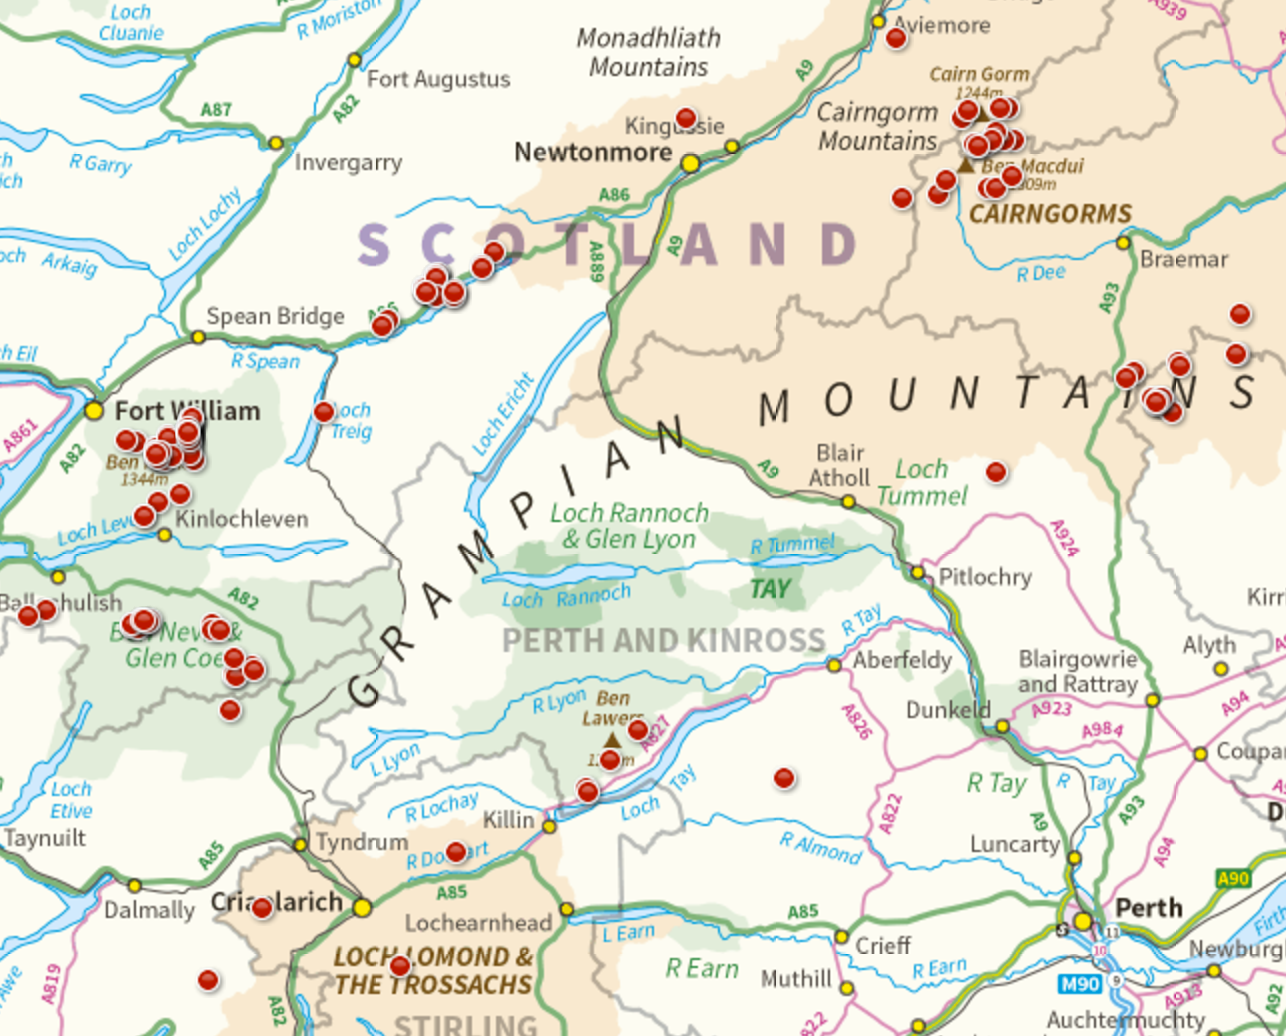
\includegraphics[scale=0.4]{ScotAvalanches1516.png}
		\caption{\label{fig:scotava1516} Reported avalanches in the Cairngorms and the Glencoe regions during winter sports season of 2015-2016, generated by the SAIS.\cite{sais-map}}
\end{figure}

The most notable application of the NN method is by the SAIS. Avalanche forecasts from the SAIS that are partially dependent on the NN method achieved a weighted accuracy of between 71\% and 82\% on visible winter days between 1998 and 2002 \cite[p. 351]{Purves2003343}. With up to 205 avalanches reported during the winter season of 2015-2016 \cite{sais} (as partly shown in Figure \ref{fig:scotava1516}), the SAIS plays a very significant role in saving lives from avalanches. Data from SAIS forecasts would also be a critical component in data sourcing and hazard modelling during this project, and is directly used to derive the hazard map overlay in \textbf{Stage 1} of the project.

In addition to analysis of snow and terrain conditions and past avalanche records, studies of vegetations in mountainous areas can also provide important information on recurrence of avalanches. Christophe \textit{et al.} \cite{Christophe2010107} developed a model based on observation of tree-rings. As avalanches affect the growth of trees and other vegetations on the mountain slopes, growth condition of trees would provide useful insight into the magnitude and frequency of past avalanches in the area. One downside of the model is its unsuitableness for direct use in forecasting temporal avalanches, as the formation of general vegetation conditions require a long period of time. However, for the purpose of this project, this model could potentially be used for establishing a static risk level for each point in the terrain, which is to be included in the overall risk model.

\section{Modelling and visualisation of avalanche hazard in GIS} \label{sec:modelling-avalanche}

In order to effective store large amounts of geographical data for computing hazard map overlays for the project, a geographic information system (GIS) \cite{clarke1986advances} is commonly used to organise avalanche hazard data.

While a majority of implemented avalanche forecasting methods -- such as those discussed in Section \ref{sec:avalanche-forecasting} -- provide generalised risk levels with respect to unique sets of environmental conditions, these generalised risk levels cannot be easily converted into localised hazards in a GIS, as these forecasting methods only operate on smaller subsets of parameters contributing to an avalanche. To evaluate the avalanche hazard of a specific location (e.g. Red Burn in Ben Nevis, Lochaber), a systematic method is often developed to calculate risk for each point in the region, taking into account as many hazard parameters as possible, which will be demonstrated by past researches discussed in this section.

According to B�hler \textit{et al.} \cite{buhler2013automated}, parameters influencing avalanche hazards can generally be placed in one of the three categories: (a) terrain topography features at each point in the modelled area; (b) meteorological data of the general area; and (c) characteristics of the snow cover in the area.

Terrain topography features, such as aspect and slope \cite[pp. 17-18]{1456186}, convexity and concavity \cite[p. 267]{de2007geospatial}, and roughness \cite[p. 12]{wilson2007multiscale} can be computed directly from a terrain height-map raster. For the main area of study in this project -- Scotland, the government-owned Ordnance Survey has mapped the entire terrain of the British Isles (excluding Republic of Ireland) into a raster with resolution of 5 meters \cite{os-5-manual}. The data is updated frequently, and has a root-mean-square error of 2.5 meters in mountainous area. The level of resolution and precision is considered as capable of producing good representations of morphologic complexity and surface topography by Rayburg \textit{et al.} \cite{Rayburg2009261}. As terrain features outside urban areas are not subject to frequent change, once the aforementioned terrain features are computed, they do not need to be re-computed until the source terrain data updates.

Meteorological and snow profile data, on the other hand, are largely dependent on the current and recent weather conditions in the forecasting regions. Commonly examined parameters by past researches include temperature change, snow accumulation \cite{WARD1984109}, humidity\cite{durand1993meteorological}, and wind direction \cite{veitinger2014slab}; as well as snow profile parameters such as snow grain size and density (as analysed in the SNOWPACK model \cite{Lehning2001253}). However, as most past researches relied on weather forecasts in the regions in which they were conducted, not all parameters they used are available in Scotland. Fortunately, each SAIS avalanche forecast is also accompanied by a snow profile, containing measured meteorological and snow conditions observed during the field work of that forecast \cite{sais-snow-profiles}. 

A number of efforts have been made to produce GIS models of avalanche hazards based on some or all of the aforementioned hazard parameters.

\begin{figure}[h]
		\centering
		\includegraphics[scale=0.5]{PreviousVisualisations.png}
		\caption{\label{fig:previous-visualisations} Hazard maps produced by prior efforts in visualising avalanche hazards: flow model and snow profile analysis by Cappabianca \textit{et al.} (top-left) \cite{Cappabianca2008193}; data-driven analysis by Pistocchi and Notarnicola (bottom-left) \cite{Pistocchi2013}; terrain topography analysis by B�hler \textit{et al.} (top-right) \cite{buhler2013automated}; and terrain topography and wind shelter analysis by Veitinger \textit{et al.} (bottom-right) \cite{veitinger2016potential}.}
\end{figure}

Gr�t-Regamey and Straub \cite{Straub2006192} utilised a Bayesian network to study the relation between snow accumulation and flow model of avalanches, and visualised risks of avalanche impacts in an area with the trained network \cite{gret2006spatially}. A more comprehensive risk model was used by Cappabianca \textit{et al.} \cite{Cappabianca2008193} to produce a similar visualisation, as shown in Figure \ref{fig:previous-visualisations} (top-left). 

However, neither of the two studies above considered the full topography features of the triggering zones (e.g. lacking convexity and terrain roughness), some of which significantly affect the probability of release, as shown by Ghinoi and Chung \cite{Ghinoi2005305}. B�hler \textit{et al.} \cite{buhler2013automated} devised a considerably accurate release zone identification algorithm based on terrain topography features alone, as visualised in Figure \ref{fig:previous-visualisations} (top-right). 

More recent researches have also included meteorological analysis in the risk model. A notable example is by Veitinger \textit{et al.} \cite{veitinger2016potential} in 2016: in addition to topography features such as slope and roughness, wind sheltering effects of the terrain was computed based on the direction of wind, and included in the fuzzy logic computations of per-point risk. The algorithm's visualisation of avalanche release risk on a slope where a real avalanche took place is shown in Figure \ref{fig:previous-visualisations} (bottom-right). While evaluations showed that little accuracy improvement was achieved in the general case due to potential mapping errors, the algorithm was more accurate than its predecessor in locating frequent avalanche release areas.

Most hazard map visualisations of the aforementioned studies are in 2D only and are static once computed, providing no interactive capabilities. To our knowledge, only Pistocchi and Notarnicola \cite{Pistocchi2013} constructed a static 3D model with an avalanche risk overlay, as shown in Figure \ref{fig:previous-visualisations} (bottom-left). The risk model by Pistocchi and Notarnicola considers a mix of static terrain features (slope, aspect, curvature, etc.), land features (forest cover) and dynamic features (snow cover duration), and deploys both Weights of Evidence and Logistic Regression to compute the avalanche release potential of each area. At best cases, this model predicts about 70\% of avalanches in the 20\% of area classified at highest hazard. 

Risk visualisations produced by all past efforts discussed in this section are static imageries. For field uses, capabilities of displaying additional image layers and map features "on the fly", as well as the ability to observe from different angles and distances could be very helpful to users.

\section{Colour representation of risks} \label{sec:colour-representation}

While a realistic imagery of the surface can be produced in the 3D viewer by covering the artificial surface with corresponding aerial photographs, an appropriate colour representation scheme needs to be chosen for the hazard map overlay, which visualises the risk level at each point in the terrain model. Considerations need to be made regarding the choice of the colour scheme, as well as in what form the colours are displayed. While all colour schemes should have an unique representation for each distinct level of risk, how well an average user of the application perceives the colour scheme is a usability issue. The two main colour schemes proposed by existing researches and some attempts of applying them will be discussed in this section.

\subsection{Saturation-based colouring}

This is the simplest colour representation scheme. A single colour determined by one hue value is chosen, and in the context of visualising hazards, the colour of choice is often red \cite{aerts2003testing} \cite{cheong2016evaluating}. The saturation of this colour at different points in the visualisation would vary, dependent on the level of risk at that point. As summarised by Cheong \textit{et al.} \cite[Ch. 2]{cheong2016evaluating}, there have been conflicting conclusions from researches on the effectiveness of saturation-based risk visualisations, when compared with visualisations using other schemes. Experiments also conducted by Cheong \textit{et al.} showed that the accuracy of user decisions under this scheme is good while multitasking, but otherwise not as good. 

While the subject of risk mapped by the visualisation of Cheong \textit{et al.} is wildfire hazard, a known visualisation of avalanche hazard under this saturation-based scheme was by B�hler \textit{et al.} \cite{buhler2013automated} as discussed in Section \ref{sec:modelling-avalanche}, although no human-computer interaction (HCI) evaluation was conducted. This scheme is also used by Spachinger \textit{et al.} \cite{spachinger2008flood} for flood risks.

\subsection{Hue-based colouring} \label{subsec:hue-based-colouring}

This colour representation scheme is similar to the saturation-based scheme, but uses different hues of colours (e.g. yellow and red) for different levels of risk in the visualisation. The European Avalanche Hazard Scale \cite[pp. 93-94]{91097820150101} -- also used by the SAIS in the UK -- applies such a hue-based scheme, as shown in Figure \ref{fig:eu-avalanche-scale}. This scheme is also used in visualisation of avalanche hazards by most studies discussed in Section \ref{sec:modelling-avalanche}, as shown in Figure \ref{fig:previous-visualisations}. 

\begin{figure}[h]
\small
\centering
\begin{tabular}{|>{\centering\arraybackslash}p{2.6cm}|>{\centering\arraybackslash}p{2.6cm}|>{\centering\arraybackslash}p{2.9cm}|>{\centering\arraybackslash}p{2.6cm}|>{\centering\arraybackslash}p{2.6cm}| } 
 \hline
 \cellcolor{low}Low Risk 
 & \cellcolor{moderate}Moderate Risk
 & \cellcolor{considerable}Considerable Risk
 & \cellcolor{high}High Risk
 & \cellcolor{veryhigh}\textcolor{white}{Very High Risk} \\
 \hline
\end{tabular}
\caption{\label{fig:eu-avalanche-scale} colour scheme reconstructed from the European Avalanche Hazard Scale, used by the SAIS \cite{sais-report}.}
\end{figure}
		
However, some studies have considered the hue-based scheme used in Figure \ref{fig:eu-avalanche-scale} to be insufficiently effective, most notably by Conger \cite{conger2004review}, who found that using green to represent low risk deviates from the common perception of green being a safe-indicator colour, which is not always the case in avalanche forecasting. Orange was also found to be sometimes inappropriate in association with a risk, and more difficult to print cartographically \cite[Ch. 4.2]{conger2004review}. Therefore Conger has suggested that the risk scale should be rescaled into four, in order to abolish the use of orange. However, other researches such as Braun and Silver \cite[p. 2212]{braun1995interaction} disagree with Conger's assessment of orange.

HCI evaluations conducted by Cheong \textit{et al.} \cite[Ch. 5]{cheong2016evaluating} concluded that while a hue-based scheme is often most preferred by users, its user decision accuracy is not the best among different colour representation schemes.
 
Other variations of applying hue-based colouring include an attempt by Gavald� and Moner \cite{gavalda2008mountaineeroriented} to represent mountaineering route hazards with red-yellow-green traffic signals; as well as a method developed by Saito \textit{et al.} \cite{saito2005two}, using two tones of hue to represent hazard at each level, which in this case is unsuitable for the steep transitions of risk frequently occurring in avalanche hazard maps \cite[Ch. 5.1]{saito2005two}. Conger \cite[Ch. 5.2]{conger2004review} also suggested a method of partially filling hazard areas with triangles that are coloured according to the colour scheme. This however would be difficult to implement in practice, due to the size variations of neighbouring points with the same risk level.

\section{Cost-based terrain pathfinding} \label{sec:terrain-pathfinding}

Based on computations of per-point risk in \textbf{Stage 2} of the project, \textbf{Stage 3} focuses on implementing the extended functionality of terrain pathfinding, which will involve adapting existing pathfinding algorithms for use under the complicated conditions of backcountry terrain.

As according to Moore \textit{et al.} \cite[pp. 4-5]{moore1991digital}, the terrain height map raster from Ordnance Survey, as discussed in \ref{sec:modelling-avalanche} is essentially a square-grid network model of the real terrain. The network model was constructed from sampling the real elevation data at a resolution of 5 meters, which minimises the risk of missing abrupt changes in elevation. Pathfinding can then be conducted on the model. The most widely implemented algorithm for this purpose is the A* Search Algorithm \cite{4082128}, utilising heuristic analysis to guide a graph search based on Dijkstra's Algorithm \cite{Dijkstra:1959:NTP:2722880.2722945}. Most practical uses of search algorithms prefer the use of A* Search to a pure implementation of Dijkstra's Algorithm, as the former's heuristic function, when well-chosen, guides the search to a far quicker (although sometimes non-optimal) arrival at the goal, particularly in a large search space.

A* is most widely implemented in the development of pathfinding artificial intelligences in computer games \cite{cui2011based}. Since its introduction, a significant number of studies have been conducted to improve the performance of A* search, including iterative-deepening A* (IDA) \cite{korf1985depth}  which requires less memory at runtime; hierarchical path-finding A* (HPA) \cite{botea2004near}, which utilises hierarchical abstraction on large data grids to produce a near-optimal solution at very high performance; and \textit{navigational mesh} (NavMesh) \cite{tozour2002building}, which minimises the structure representation of data to reduce memory use and computation time. However, the hierarchical structure of HPA means that interconnection points between sub-level grids are often picked around obstacles, which do not exist on the elevation-based terrain grid, potentially hindering HPA's performance if applied.

When adapting A* or its aforementioned variants for computing a path in the terrain and taking into account the avalanche risk level at each point in the terrain raster, both the distance and the risk levels need to considered by the heuristic function of A*. Due to the nature of the uneven terrain, the proper walking distances between points can be estimated by Naismith's Rule and its variants \cite{magyari2012determining}. The accuracy of this estimation decreases as the resolution of the terrain raster decreases, which can occur if the terrain has to be down-sampled to reduce search space size.

To represent the points as a data structure, Yap \cite{yap2002grid} has suggested using a tiled hex grid to organise neighbouring points for optimisation of performance, which then be analysed with a hierarchical search algorithm such as HPA \cite{botea2004near}. However, it is relatively difficult to re-project square grids of the terrain model into hex tiles, as terrain feature displacements can occur.

\section{Usability aspects of the application} \label{sec:application-usability}

As the project requires that the front-end application to be built is usable both on a mobile device with touchscreen and on a desktop computer with a mouse, best practises of design from existing HCI research on both types of user interfaces need to be considered, as well as the principles for a system that would potentially be used in the field rather than in office.

Nielson and Olsen \cite{nielson1987direct} proposed a formal method of manipulating the view of a 3D object (such as the virtual terrain globe in this application) with a 2D interface. This allows translations, rotations and scalings of the object to be performed by a single 2D event device, such as a mouse. In practise, methods of interactions have been mapped to specific combinations of actions of the mouse wheel and mouse keys \cite[pp. 195-197]{haklay2010interacting}. However, not all users find mouse interactions straightforward when navigating a 3D scene, and their satisfaction of the mouse interface largely depends on their proficiency with the mouse, as demonstrated by Dubois \textit{et al.} \cite{Dubois:2007:EAI:1531407.1531416}. 

On modern mobile devices, touchscreen is often the only interface available for the user to interact with the application. With mouse clicks replaced by touch interactions \cite[p. 191]{haklay2010interacting}, manipulations of the 3D object in the viewer are often less straightforward, as studied by Ku and Chen \cite{ku2014study}, which provided some recommendations on designing touchscreen-based interactions of a 3D object viewer. 

For an application that could be used in the field under time and user attention constraints, a study by Pascoe \textit{et al.} \cite{pascoe2000using} shows that the application should have context awareness and utilise interaction designs which minimise distraction to the user. Another study by Albinsson and Zhai \cite{Albinsson:2003:HPT:642611.642631} explored methods to improve the precision of touchscreen interactions under rough inputs from human fingers.
 
\chapter{Theories and Methodologies} \label{ch:theory}

This chapter provides the details of the theories in avalanche forecasting, spatial analysis, risk representation and search algorithms applied across different stages of the project. Section \ref{sec:dynamic-factors} will be utilised in the construction of basic functionalities in \textbf{Stage 1}, which is improved in \textbf{Stage 2} with the introduction of Sections \ref{sec:static-factors} and \ref{sec:chosen-colour-coding}. Section \ref{sec:risky-pathfinding} provides the basis of algorithm design and implementation in \textbf{Stage 3}. Finally, Section \ref{sec:stats-eval} provides theoretical basis of statistically evaluating the risk model devised against past efforts in \textbf{Stage 4} .

\section{Dynamic risk factors of avalanche release} \label{sec:dynamic-factors}

Dynamic factors in avalanche forecasting are considered as factors that change over time, including but not limited to snow precipitation, conditions of snow cover (both well-studied by SNOWPACK \cite{Lehning2001253} as described in Section \ref{sec:avalanche-forecasting}), air temperature, wind direction and windspeed (studied by Veitinger \textit{et al.} \cite{veitinger2016potential} as described in Section \ref{sec:modelling-avalanche}). These factors also form the major elements of the Nearest Neighbour (NN) forecasting method (\ref{sec:avalanche-forecasting}), which is used by the project's source of dynamic risk data -- the Scottish Avalanche Information Service (SAIS). 

Purves \textit{et al.} \cite{Purves2003343} described the process utilised by the SAIS to forecast avalanche risk in Scottish mountains. Through an NN modelling software tracking observed past avalanches, forecasters will input measurements on temperature, wind and snow conditions, which are then scaled to the same range, and weighted by an autonomous genetic algorithm in order to avoid overfitting on recent avalanche conditions. This process creates a vector in the NN vector-space. The software then provides the input vector's nearest neighbours, the conditions of which then allows experienced forecasters to make a decision on the level of risk for each segment of aspect and altitude in each region. The resulting compass rose-style diagram can be seen in Figure \ref{fig:mapping}.

Based on the existing evaluations of the accuracy of SAIS avalanche forecasts \cite[p. 351]{Purves2003343} \cite{heierli2004verification}, with an accuracy of above 70\% on clear winter days, we have confidence that the dynamic risk model used by the SAIS provides a relatively reliable overview of dynamic avalanche risks across different aspects and altitudes, through a composition of different dynamic factors available to the SAIS observers. Therefore, SAIS risk data were applied directly to the terrain model for the basic application developed in \textbf{Stage 1}.

\section{Static risk factors of avalanche release} \label{sec:static-factors} % Surface fitting.

Static factors in avalanche forecasting mainly concern the terrain topographic features that rarely change over time. Based on a height map of the terrain, various features can be computed through mathematical formulations. As summarised in Section \ref{sec:modelling-avalanche}, past efforts in modelling avalanche risks based on terrain features have generally covered the following features: altitude, slope, terrain curvature (convexities and concavities) and aspect. While past researches such as Ghinoi and Chung \cite[p. 313]{Ghinoi2005305} have attempted to reclassify altitudes data into distinct altitude bands to take into account the effects of altitude on avalanche risks, this has been equivalently considered in the dynamic risk model (\ref{sec:dynamic-factors}). Therefore, only slope, curvature and aspect are considered in the static risk model of this project. 

\subsection{Surface fitting with a 2nd order polynomial}

By definition, slope, curvature and aspect are topography properties relative to a point's neighbourhood, usually within a window of 8 surrounding points in a rectangular grid. Therefore, to calculate these properties for each point, it is necessary to fit a polynomial surface within each such neighbourhood. A commonly used process is to fit a second degree polynomial surface to the neighbourhood. While it is generally agreed that a 2nd order polynomial is the most suitable for the 9-point 3D surface \cite{zevenbergen1987quantitative} \cite{heerdegen1982quantifying} \cite{evans1979integrated}, past efforts have applied different configurations of parameters. The configuration chosen for this project is a 9-parameter polynomial by Zevenbergen and Thorne \cite[p. 49]{heerdegen1982quantifying}, which has an order of 2 in each of the x and y directions, as shown in \ref{eq:surface-polynomial}. This model has the advantage of accurately passing through each point in the neighbourhood with uniquely determined parameters \cite[Sec. 6.1.3]{de2007geospatial}.

\begin{equation} \label{eq:surface-polynomial}
Z = Ax^{2}y^{2} + Bx^{2}y + Cxy^{2}+Dx^{2} + Ey^{2} + Fxy + Gx + Hy + I
\end{equation}

Where coefficients \textit{A} to \textit{I} are determined by solving a linear system of equations between coordinates of (\textit{x}, \textit{y}) and known \textit{Z} values in the height map. The point where the neighbourhood is centered on is (0, 0), and the grid is expressed as followed:

\begin{center}
\begin{tabular}{ccc}
(-1,1) & (0,1) & (1,1) \\
(-1,0) & (0,0) & (1,0) \\
(-1,-1) & (0,-1) & (1,-1) \\
\end{tabular}
\end{center}

As the center pixel (0, 0) is the point where we would like to determine the values of slope, curvature and aspect, which are all derived from the first or second derivatives of the surface polynomial \cite[p. 312]{Ghinoi2005305}. Only constant terms in the derivatives will be required for the calculations, as explained in \ref{subsec:slope}, \ref{subsec:curvature} and \ref{subsec:roughness}.

\subsection{Modelling avalanche risk from slope} \label{subsec:slope}

The slope angle represents the steepness of the terrain at a point, which can be determined by calculating the magnitude of change (first derivative) in both directions \cite[p. 50]{zevenbergen1987quantitative}. Practically, negation is applied to the value to represent that the slope is down-hill, but this is not required in modelling avalanche risk.

The first order partial derivatives of the surface polynomial described in \ref{eq:surface-polynomial} are as followed:

\begin{equation} \label{eq:first-derivatives}
\begin{aligned}
\frac{\partial{Z}}{\partial{x}} = 2Axy^{2} + 2Bxy + Cy^{2} + 2Dx + Fy + G \\
\frac{\partial{Z}}{\partial{y}} = 2Ax^{2}y + Bx^{2} + 2Cxy + 2Ey + Fx + H
\end{aligned}
\end{equation}

At the center point where the slope angle value is required, with coordinates (0, 0), it is trivial to determine the magnitude of change:
\begin{equation} \label{eq:first-derivatives-zeros}
\begin{aligned}
&When \   x = 0,\ y = 0: \\
&\frac{\partial{Z}}{\partial{x}} =  G, \   \frac{\partial{Z}}{\partial{y}} = H \\
&\Rightarrow SLOPE = \sqrt{G^{2} + H^{2}}
\end{aligned}
\end{equation}

According to Horn \cite{1456186}, the slope angle is simply the inverse tangent of the magnitude in degree form: 
\begin{equation}
S_t = \tan ^{ - 1} (SLOPE) = \tan ^{ - 1}(\sqrt{G^{2} + H^{2}})
\end{equation}

The consensus of most researches is that the majority of avalanches occur between a slope angle range of 25\degree \ and 60\degree, with the highest level of risk near the middle of the range \cite[p. 42]{91097820150101}\cite[p. 112]{mcclung2006avalanche}. Veitinger and Sovilla \cite[p. 2215]{veitinger2016potential} modelled this observation as a bell-shaped curve, which has been adapted by our model. The modification our model made to the curve from the original was moving the symmetrical line in x direction to \textit{x} = 42.5\degree \ to make the curve fit better with the McClung \cite[p. 112]{mcclung2006avalanche} model, as shown in Figure \ref{fig:slope-curve}.

\begin{figure}[h]
		\centering
		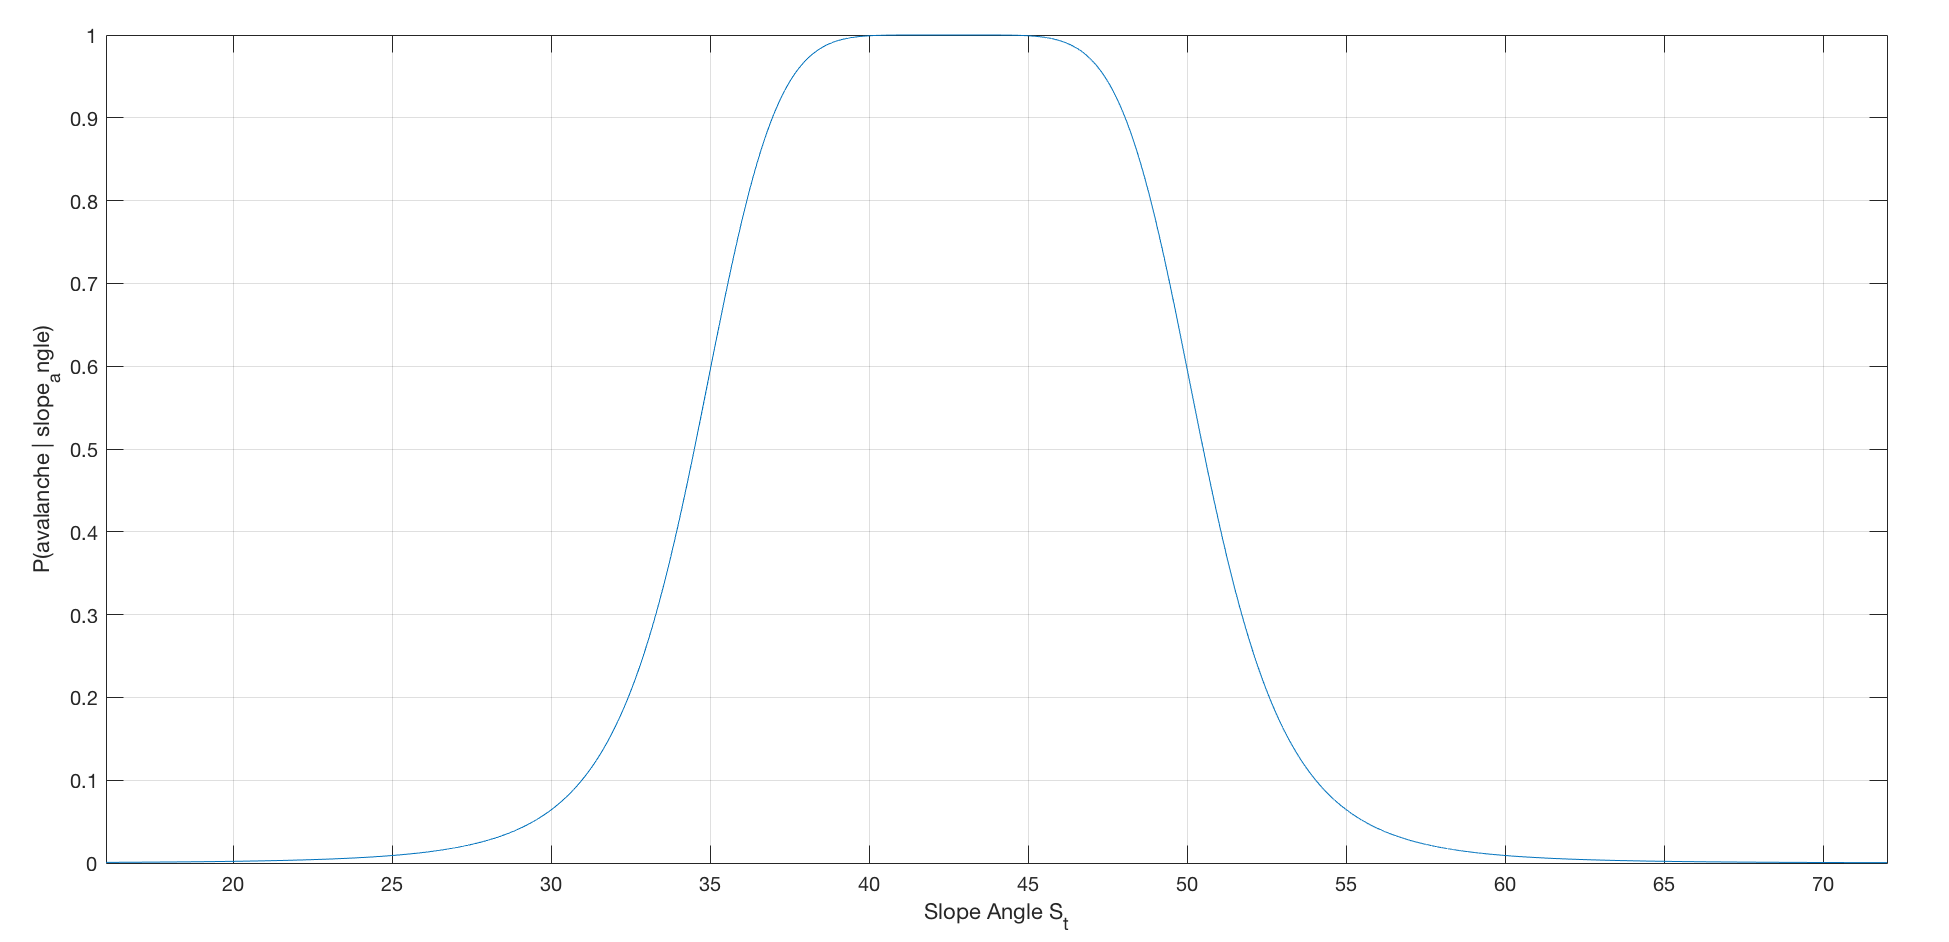
\includegraphics[height=5cm]{slope-curve.png}
		\begin{equation} \label{eq:slope-curve}
		R_s = \frac{1}{(1+(\frac{x-42.5}{8})^{6})}
		\end{equation}
		\caption{\label{fig:slope-curve} Adapted bell-shaped curve for modelling avalanche risk of slope angles.}
\end{figure}

\subsection{Modelling avalanche risk from curvature} \label{subsec:curvature}

Another significant static influence on the risk of avalanche release is terrain curvature, which can either be convex, concave or linear, as shown in  \ref{fig:convex-concave}. Along the vertical and the horizontal plane, there are two different types of terrain curvatures: profile curvature and planform curvature \cite[p. 50]{zevenbergen1987quantitative}. As the release of avalanches are mainly concerned with gravity in vertical plane, only the profile curvature is considered in our risk model.

\begin{figure}[h]
		\centering
		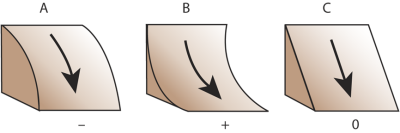
\includegraphics[height=3cm]{convex-concave.png}
		\caption{\label{fig:convex-concave} An illustration of concave (A), convex (B) and linear (C) terrains. \cite[p. 360]{menno2013map}}
\end{figure}

In conformance with the convention, our model defines the value of the profile curvature as one over the radius of the neighbourhood curvature in meters. As with illustrated in Figure \ref{fig:convex-concave}, concave curvatures are expressed as negative, convex curvatures are expressed as positive, while linear terrain is defined to have a curvature value of zero. 

As observed by McClung \cite[p. 115]{mcclung2006avalanche}, a majority of avalanches occur on terrains that are without significant curvature (forming a region of similar risk levels near a curvature value of zero), and convex terrains tend to increase the probability of slab avalanches by gliding. Conversely, snowpacks taper off on concave slopes, which reduces the probability of slab avalanches. Therefore, we produced a new curve for our model in modelling avalanche risk from curvature, as shown in Figure \ref{fig:curvature-curve}.

\begin{figure}[h]
		\centering
		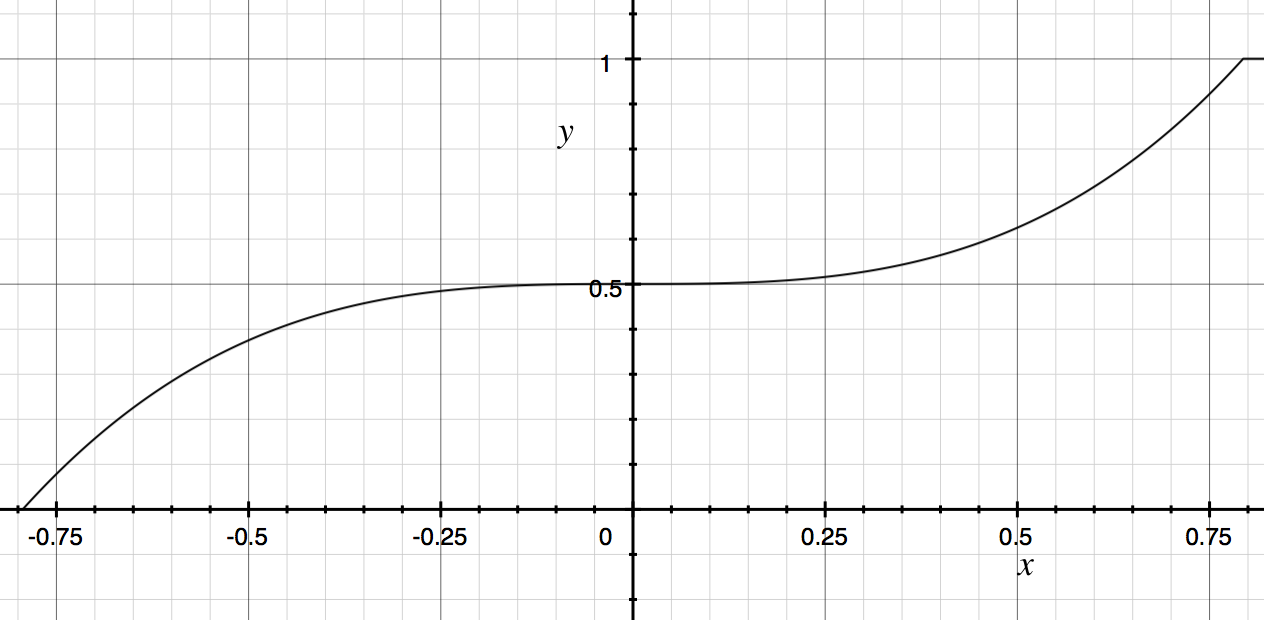
\includegraphics[height=5cm]{curvature-curve.png}
\begin{equation} \label{eq:curvature-curve}
  R_c =
  \begin{cases}
    x^3 + 0.5 & -0.7937 \leq x \leq 0.7937 \\
    1 & x > 0.7937 \\
    0 & \text{otherwise}
  \end{cases}
\end{equation}
\caption{\label{fig:curvature-curve} A spline for modelling avalanche risk of terrain curvature.}
\end{figure}

As shown by (\ref{eq:curvature-curve}), the numerical model of the spline is based on the curve of function $y = x^3 + 0.5$, but with a range of $[0, 1]$ to form a numerically-valid risk factor. Extreme curvatures represented by $x > 0.7937$ or $x < -0.7937$ (curvature radius $r < 1.26m$) will be capped at extreme risk values $R_c = 1$ and $R_c = 0$ respectively. We believe that the shape of the spline models the aforementioned effects of changing terrain curvature well: as the terrain levels off from a concave, the avalanche risk increases steeply until approaching the linear region, where there is no significance change in the risk level; and as the terrain curvature increases away from this region into convex, the avalanche risk increases again steeply.

In practise, the curvature value $x$ can be easily computed by taking the second derivative of (\ref{eq:surface-polynomial}) with respect to the aspect angle (calculated by $\theta = atan(\frac{H}{G})$) in the fitted neighbourhood, which is:

\begin{equation} \label{eq:curvature-equation}
x = \frac{-2(DG^2+EH^2+FGH)}{G^2+H^2}
\end{equation}

\subsection{Modelling avalanche risk from terrain roughness based on aspect and slope} \label{subsec:roughness}

While slope angle and curvature have a direct influence on the risk of avalanche release \cite[p. 1311]{buhler2013automated}, aspect angle does not hold a significance in avalanche risk itself, as it only indicates the direction in horizontal plane the terrain is facing. Instead, aspect angle is used in conjunction with slope angle to calculate the roughness of the terrain, which measures the mechanical resistance of the terrain on the snow cover. The higher the mechanical resistance, the harder it is for a large scale avalanche to be released \cite[p. 313]{Ghinoi2005305}.

There are various methods for calculating a terrain roughness index, some of which involves the consideration of landcover, which may change between seasons. Other factors such as changes in vegetation due to planting and logging may also affect the accuracy of a roughness index calculated from landcover data. Therefore, an alternative method based on elevation can be used. A notable method based on vector dispersion, originally developed by Sappington \textit{et al.} \cite{sappington2007quantifying} and improved by Veitinger and Sovilla \cite[p. 2216]{veitinger2016potential} can be used.

The method works by decomposing the fitted neighbourhood of nine points into three components ($X$, $Y$ and $Z$) based on the values of slope angle ($\alpha$) and aspect ($\beta$) at each point. Then for each of the three components, we sum up the neighbourhood. A resulting vector |r| can then be calculated for the center point by further sum up the squares of the three neighbourhood sums and taking the square root. Finally, the roughness index $R$ can be determined by normalising the vector with the number of points in the neighbourhood (that is, 9) and subtract it from 1. The process is shown as followed:

\begin{equation}\label{eq:roughness-equation}
\begin{aligned}
d_{xy} &= 1 \cdot sin(\alpha) \\ &\Rightarrow Z = 1 \cdot cos(\alpha),\  X = d_{xy} \cdot cos(\beta),\  Y = d_{xy} \cdot sin(\beta) \\
|r| &= \sqrt{(\sum X)^2 + (\sum Y) ^ 2 + (\sum Z) ^ 2} \\
x_r &= 1 - \frac{|r|}{9}
\end{aligned}
\end{equation}

From (\ref{eq:roughness-equation}), it is easily observed that the value of $x_r$ is always positive. The tested model by Veitinger and Sovilla \cite[p. 2216]{veitinger2016potential} believes that avalanche risk decreases sharply between 0 and 0.01, and further decreases slowly between 0.01 and 0.02. At a roughness level of above 0.02, an avalanche release will be unlikely. Therefore, a similar bell shaped curve is used as shown in Figure \ref{fig:roughness-curve}, albeit only using the relevant section where $x_r > 0$.

\begin{figure}[h]
		\centering
		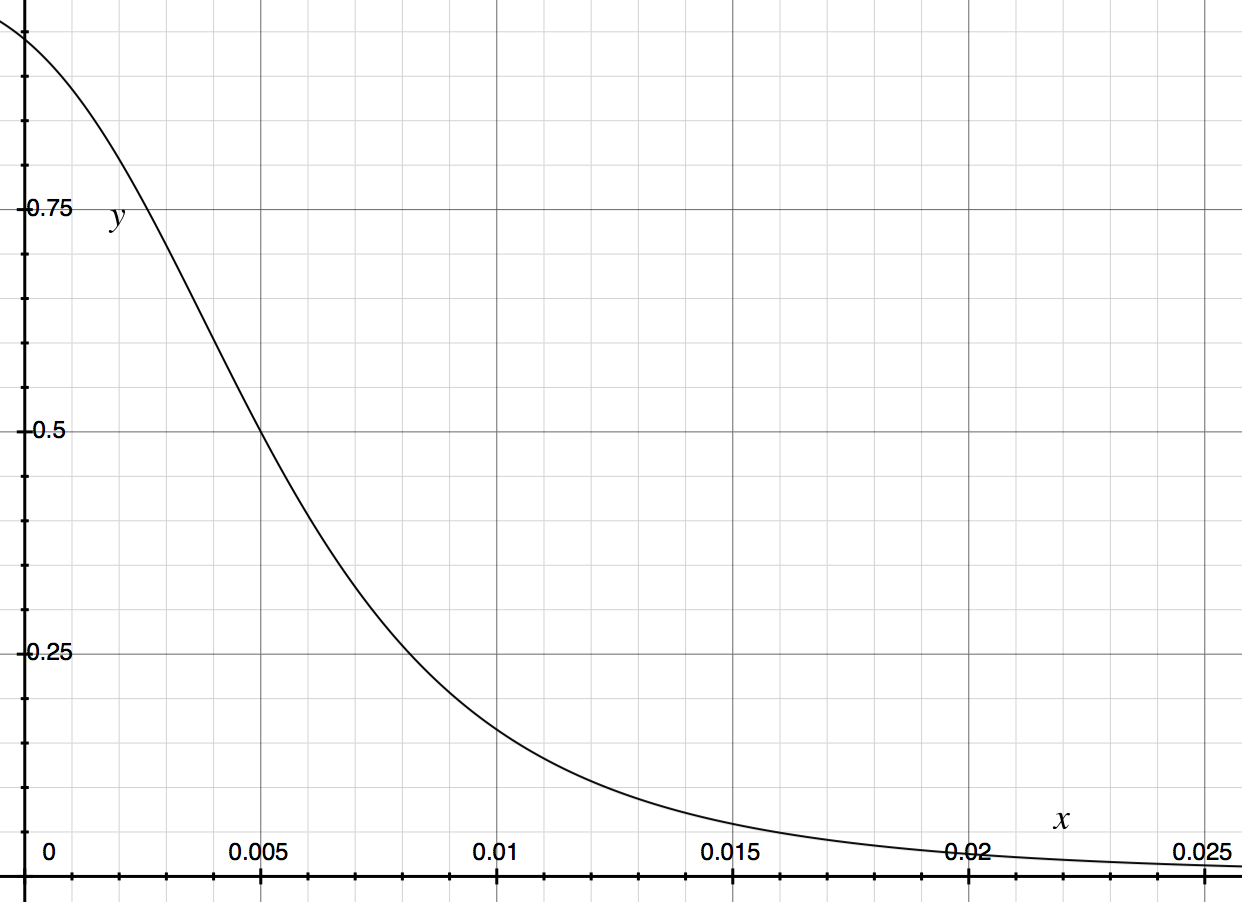
\includegraphics[height=6cm]{roughness-curve.png}
\begin{equation} \label{eq:roughness-curve}
R_r = \frac{1}{(1+(\frac{x_r+0.005}{0.01})^{4})}
\end{equation}
\caption{\label{fig:roughness-curve} A bell-shaped curve for modelling avalanche risk of terrain roughness index.}
\end{figure}

\subsection{Combining static risk models}

With three different static risk factors calculated: slope angle, curvature and roughness, a method of uniforming the three into a single per-point risk value is needed. While it is possible to apply a Support Vector Machine (SVM) \cite{pozdnoukhov2011spatio} as described in Section \ref{sec:avalanche-forecasting} or a fuzzy logic operator \cite[p. 2218]{veitinger2016potential}, because all three static risk factors are in the range of $[0, 1]$ and all represent a linear risk scale, the most efficient way to combine them is to multiply the three risk factors at each point together after normalising them. This also has the advantage of avoiding potential biases caused by the choice of weighting factors in a SVM or fuzzy operator.

In order to determine the normalising constant, the integral of $x$ is calculated from each of the three models: the risk curve of slope angles (\ref{eq:slope-curve}), the risk spline of terrain curvature (\ref{eq:curvature-curve}), and the risk curve of terrain roughness index (\ref{eq:roughness-curve}); with intervals $[0, 90]$ (valid slope angles in degrees), $[-0.7937, 0.7937]$ (uncapped range of terrain curvature), and $[0, \infty]$ (valid roughness index values) respectively. Values of each risk factor at each point is divided by its normalising constant, and then multiplied together at each point. The process is shown as followed:

\begin{equation}\label{eq:combining-static-risk}
R_{combined} = \frac{R_s}{C_s} \cdot \frac{R_c}{C_c} \cdot \frac{R_r}{C_r} 
\end{equation}

Where $R_s$, $R_c$ and $R_r$  are risk factors for slope, curvature and roughness respectively, and $C_s$, $C_c$ and $C_r$  are their normalising constants.

\section{Colour visualisation of risk} \label{sec:chosen-colour-coding} % Explain change of colour coding first.

For the basic application completed in \textbf{Stage 1}, a colour scheme identical to the colour coding used by the SAIS (as shown in Figure \ref{fig:eu-avalanche-scale}) was used for the risk levels (which at \textbf{Stage 1} relies only on the dynamic risk model). However, as described in Section \ref{sec:colour-representation}, past researches have found this colour coding scheme to be ineffective and has the potential to mislead the user. Therefore, a new colour scheme was implemented, as shown in Figure \ref{fig:new-avalanche-scale}.

\begin{figure}[h]
\small
\centering
\begin{tabular}{|>{\centering\arraybackslash}p{2.6cm}|>{\centering\arraybackslash}p{2.6cm}|>{\centering\arraybackslash}p{2.9cm}|>{\centering\arraybackslash}p{2.6cm}|>{\centering\arraybackslash}p{2.6cm}| } 
 \hline
 \cellcolor{low-new}Low Risk
 & \cellcolor{moderate-new}Moderate Risk
 & \cellcolor{considerable-new}Considerable Risk
 & \cellcolor{high-new}\textcolor{white}{High Risk}
 & \cellcolor{veryhigh-new}\textcolor{white}{Very High Risk} \\
 \hline
\end{tabular}
\caption{\label{fig:new-avalanche-scale} The new colour scheme implemented in \textbf{Stage 2}.}
\end{figure}

Recommendations made by Conger \cite{conger2004review} was partially applied: green has been eliminated from the colour scheme to avoid giving the user a false perception of safety; however, the recommendation to eliminate orange was not applied, due to inconsistency of findings on orange between past researches, and orange's wide usage in risk colour codings. 

With the elimination of green, yellow is instead used for representing the low risk level, while a new risk colour with a hue value between yellow and orange, but lower lightness than both in the HSL scale is used for representing moderate risk. The hue values for other risk colourings were also slightly adjusted to produce a good distinction between different colours, the effect of which can be seen in Figure \ref{fig:stage1bennevis} (right).

\section{Combining the static risk model and the dynamic risk model} 

As shown in Figure \ref{fig:eu-avalanche-scale}, the dynamic risk model produced by the SAIS has five distinct bands of risk levels (six if the grey data-not-available is included). In contrast, as shown in Section \ref{sec:static-factors}, the static risk model contains continuous data. This requires an appropriate method to combine the two models for visualisation purposes in the application. While it is possible to merge the two models numerically again through either a Support Vector Machine (SVM) or a fuzzy logic operator, due to the lack of an established precedence between the influence of the static model and the dynamic model used in this project, the use of different representations for the two models was instead preferred. 

As described in Section \ref{sec:colour-representation}, the two main schemes for colour representation of risk are saturation-based and hue-based. This provides an opportunity for implementing a mixed approach, in which two different representations can be used: one with hue and the other with saturation. 

In particular, the dynamic risk level will determine the value of hue at a point, thus determining the "colour" of the point in the traditional sense, which is in turn determined by its altitude and terrain aspect as intended by the SAIS. The static risk level will then determine the saturation at that point. This means that the less likely static risk analysis believes that an avalanche release could occur at a point, the fainter the colour of that point will be. Conversely, a strong colour implies a high likelihood of avalanche release at a point based on static risk analysis.

In practise, thresholding will be applied to all static risk levels in the raster for the scaling of static risk value to saturation. To reduce the influence of extreme values on the visualisation of static risk, the static risk values are scaled between the 1st percentile and the 99th percentile rather than between the minimum and maximum risk values.

The resulting risk colour scheme, used by the improved application of \textbf{Stage 2}, can be seen in Figure \ref{fig:final-colour-scheme}. The effects of static risk controlling saturation can also be observed in Figure \ref{fig:stage1bennevis} (right). 

\begin{figure}[h]
		\centering
		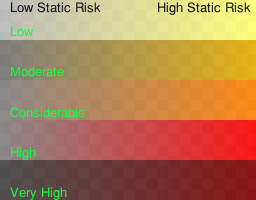
\includegraphics[height=5cm]{final-colour-scheme.png}
		\caption{\label{fig:final-colour-scheme} The new risk colour scheme implemented in the improved application. Each row represents a dynamic risk level.}
\end{figure}

\section{A* pathfinding in a risk-adjusted environment} \label{sec:risky-pathfinding}

As described in Section \ref{sec:terrain-pathfinding}, A* search is a well-studied algorithm for pathfinding in a graph, especially in challenging conditions such as large datasets and strict or real-time timing constraints. It has been chosen as the basis for the pathfinding feature in \textbf{Stage 3} over a simpler implementation of Dijkstra's Algorithm, due to the convenience of introducing avalanche risk into the former's heuristic function, as well as former's usually superior performance \cite{goldberg2005computing} when only an approximate answer is required.

There are nevertheless a number of challenges when adapting A* search for the specific purpose of risk-adjusted pathfinding in a 3D terrain, including calculating the vertical distance between two points, balancing costs in distance and risk as required, and devising a suitable heuristic function for the problem. These will be addressed in the next few subsections, followed by an overview of the adapted algorithm. 

\subsection{Vertical distance between two points}

As the height map raster available to the application arranges data in a grid with uniform resolution, vertical distances between neighbouring nodes are consistent. Therefore, the only distinction of distance between two neighbouring nodes is the vertical distance. While it is possible to calculate the linear distance between two points based on trigonometry, this is both computationally expensive for a large data grid and inaccurate: it is unlikely that the terrain surface is smooth and straight between two neighbouring points. As an alternative, it is possible to estimate this distance based on observations and average cases: the Naismith's Rule, as introduced in \ref{sec:terrain-pathfinding}.

The Naismith's Rule estimates the amount of equivalent distance walked by a mountaineer to ascend or descend each unit of vertical distance, called the Naismith distance. In average case on a natural terrain, it has been estimated that walking on a levelled terrain for 3 miles is equivalent to ascending or descending 2000 feet vertically, which is equivalent to 7.92 meters of walking distance for each meter of vertical distance, as summarised by Scarf \cite{scarf2008mathematical}. This allows a simple conversion process to be established as followed:

\begin{equation} \label{eq:naismith-equation}
\begin{aligned}
Naismith\_Distance(NodeA,\ NodeB) &= Raster\_Resolution(NodeA,\ NodeB) \\
&+ 7.92 * | NodeA.height - NodeB.height | \\
\text{where Raster\_Resolution returns the }&\text{raster resolution in the direction of PointA} \\
\text{to PointB, which is either straight or }&\text{diagonal.} 
\end{aligned}
\end{equation}

\subsection{Balancing costs in distance and risk}

A requirement of the project requires the algorithm to accept a user-configurable weighting of risk against distance, allowing the user to receive several possible routes between two points based on the importance they give to the risk enroute and the overall distance. After the user has requested a path with such a risk weighting, the application needs to calculate the overall cost of moving between two nodes accordingly. The risk weighting is between 0 and 1, representing the percentage of overall cost attributed to avalanche risk.

While it is simple to multiply the separately calculated distance cost and avalanche risk cost by their defined weights, it is also important that the two costs are normalised into the same scale before combining them. This requires the maximum and minimum distance cost and avalanche risk cost to be calculated beforehand. The full process is shown as followed:

\begin{equation} \label{eq:risk-weighting-equation}
\begin{aligned}
normalised\_distance &= \frac{Naismith\_Distance(NodeA,\ NodeB) - min\_distance}{max\_distance - min\_distance} \\
normalised\_risk &= \frac{NodeB.risk - min\_risk}{max\_risk - min\_risk} \\
overall\_movement\_cost &= normalised\_risk \cdot risk\_weighting \\
&+ normalised\_distance \cdot (1 - risk\_weighting)
\end{aligned}
\end{equation}

It is worth noting that the avalanche risk of moving between two nodes is dependent on the target node only, as calculating a potentially negative difference in risk levels between two nodes could affect the admissibility of the heuristic function.

\subsection{Heuristic function for risk-adjusted A* search}

The heuristic function used to determine the priority under which each node is explored considers not only the Naismith distance between the candidate node and the goal node, but also the immediate static risk of moving to the candidate node from the current node. The latter creates a risk-averse behaviour for the algorithm, which helps the pathfinding to avoid localised avalanche hotspots.

Due to the fact that the search will be conducted on a rectangular section of the data grid whose position is determined by the location of the start node and the goal node, and that it is possible to move diagonally in the real world, the commonly used goal distance estimation based on the Manhattan Distance must be altered, as shown in Figure \ref{fig:heuristic-distance}. 

\begin{figure}[h]
		\centering
		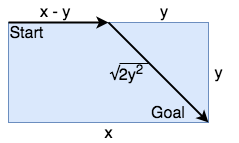
\includegraphics[height=3cm]{heuristic.png}
		\begin{equation}\label{eq:heuristic-equation}
		\begin{aligned}
		estimated\_distance &=  (x - y) + \sqrt{2 \cdot y^2} \\
		&+ 7.92 * | NextNode.height - GoalNode.height | \\
		heuristic\_cost &= estimated\_distance \cdot GoalNode.risk \\
		scaled\_heuristic &= \frac{heuristic\_cost - min\_naismith}{max\_naismith - min\_naismith}
		\end{aligned}
		\end{equation}
		\caption{\label{fig:heuristic-distance} Calculating the scaled heuristic cost.}
\end{figure}

The heuristic cost of moving to a node can then be calculated by multiplying the risk level of the next node with the estimated Naismith distance to the goal node. The resulting heuristic cost is then scaled to be between the maximum and minimum actual Naismith distances calculated. This combines with the actual cost of moving to the node, as shown in (\ref{eq:heuristic-equation}).

\subsection{Overview of the adapted A* algorithm}

\begin{algorithm}
\label{alg:a-star}
\begin{algorithmic}[1]
\State $search\_queue\gets$ PriorityQueue()
\State $search\_queue$.push(priority $\gets$ 0, $initial\_node$)
\State $source\_index\gets$ \{\}
\State $costs\_dict\gets$ \{\}
\State $source\_index[initial\_node]\gets$ None
\State $costs\_dict[inital\_node]\gets$ 0
\While{$search\_queue \not=$ empty} 
    \State $current\_node \gets$ $search\_queue$.pop();
    \If{$current\_node = goal\_node$}
         \Comment{Goal found, terminate.}
        \State break
    \EndIf
    \State $neighbours\gets$ get\_neighbours($current\_node$)
    \ForAll{$neighbour\_node \In neighbours$}
        \State $cost\gets$ naismith\_distance($current\_node$, $neighbour\_node$) * (1 - $risk\_weighting$) + $neighbour\_node$.risk * $risk\_weighting$;
        \State $new\_cost\gets$ $costs\_dict[current\_node]$ + $cost$;
        \If{$neighbour\_node \NotIn costs\_dict \Or new\_cost < costs\_dict[neighbour\_node]$}
            \State $costs\_dict[neighbour\_node]\gets$ $new\_cost$ \Comment{A shorter path.}
            \State $neighbour\_priority\gets$ $new\_cost$ + heuristic($neighbour\_node$, $goal\_node$)
            \State $search\_queue$.push(priority $\gets$ $neighbour\_priority$, $neighbour\_node$)
            \State $source\_index[neighbour\_node]\gets$ $current\_node$
        \EndIf
    \EndFor
\EndWhile
\State reconstruct\_path($goal\_node$, $source\_index$);
\end{algorithmic}
\caption{Pseudocode for the adapted A* search algorithm.}
\end{algorithm}

\begin{figure}[h]
		\centering
		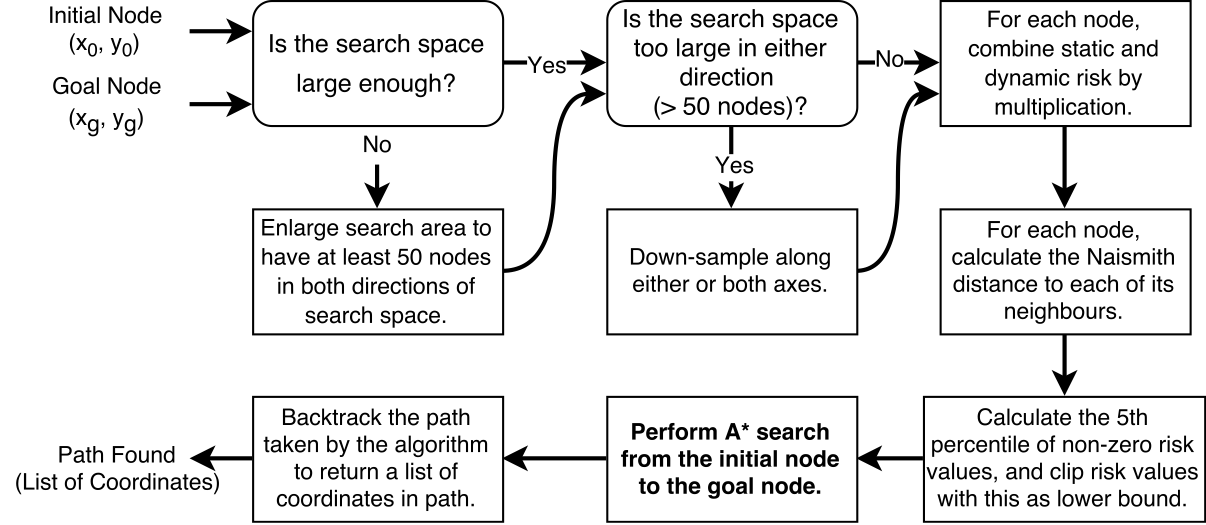
\includegraphics[height=6cm]{a-star.png}
		\caption{\label{fig:a-star} The operations of the pathfinder implementation.}
\end{figure}

As shown in Figure \ref{fig:a-star}, a few pre-processing steps are required to ensure that the algorithm can finish timely with a meaningful result. If the bounding box created by the initial and final node coordinates is too small (occurs when the line between two nodes is almost in parallel with a longitude or latitude line), the search area is enlarged to allow the algorithm more choices. If the search space is too large, linear down-sampling is applied, picking the maximum height and risk level in the sample (for conservative estimations of Naismith distance and risk), and the mean aspect angle in the sample. 

Thereafter, the Naismith distances from each node to its neighbours are calculated by applying (\ref{eq:naismith-equation}). A clipping of risk values to between the 5th percentile of non-zero risk values and the maximum risk is also conducted, as preliminary testing of the implementation showed that blocks of zero risk values significantly reduce the performance of the algorithm. 

Finally, the A* search algorithm is performed on the pre-procesed search space. A path in the form of a list of coordinates can then be constructed through backtracking the search space from the goal node.

\section{Statistical evaluation of forecast accuracy} \label{sec:stats-eval}

In order to determine the quality of the avalanche risk models used by the project, it is essential to conduct some statistical tests on the model. An ordinary approach is to conduct an inferential statistical test such as the Mann-Whitney U test \cite{mann1947test} to determine whether our models accurately determines the locations of actual avalanche releases. However, the unique design of the models and how they are combined have made applying inferential statistics difficult.

As described in Section \ref{sec:dynamic-factors}, the dynamic risk model was individually evaluated as a Nearest Neighbour model \cite[p. 351]{Purves2003343}, and was used without modification in this project. The static risk model as described in Section \ref{sec:static-factors} however uses a separate representation, and was not merged with the dynamic risk model. As there is no prior static risk model applied to the Scottish Highlands that we are aware of, it is not possible to compare the static risk model along with another model through inferential statistics. 

On the other hand, comparing the static model alone against the dynamic model also makes little sense, as the avalanche risk factors considered by the two models are largely disjoint. However, since all of these factors are critical to accurately forecasting avalanches (as described in Sections \ref{sec:avalanche-forecasting} and \ref{sec:modelling-avalanche}), demonstrating whether one model is better than the other cannot demonstrate the effectiveness of our overall model.

Therefore, a simpler statistical test can be designed. Based on the avalanche records marked by the SAIS \cite{sais-map}, avalanches that happened sufficiently close to a point with a high avalanche risk level will be recorded as a successful forecast, and vice versa. Both the threshold for the proximity of a point and for the avalanche risk level can be adjusted for multiple observations. % Talk about problems with avalanche map in evaluation section.

\chapter{Description of the Application} \label{ch:app-description}

\chapter{Evaluation and Testing of the Application} \label{ch:app-testing}

\chapter{Conclusions} \label{ch:conclusions}

\small{\bibliography{project}}
\end{document}  